La búsqueda binaria con índice invertido (BSII, \textit{Binary Search with Inverted Index}) es una evolución de la búsqueda binaria presentada previamente. Como su nombre lo indica, esta aproximación al problema de búsqueda de información utiliza un índice invertido: una estructura de datos donde se relaciona cada término del vocabulario con los documentos donde está presente. En este sentido, cada término va a estar vinculado con lo que se conoce como una lista de posteo (\textit{posting list}) donde cada ítem de dicha lista es el identificador de un documento donde aparece el término. Con el fin de optimizar el proceso de recuperación de la información se suele incluir la frecuencia relativa de cada término dentro del índice invertido. La figura \ref{fig:inverted_index} presenta una representación de un índice invertido, donde se pueden evidenciar los términos, la frecuencia relativa y la lista de posteo.

\begin{figure}[ht]
    \centering
    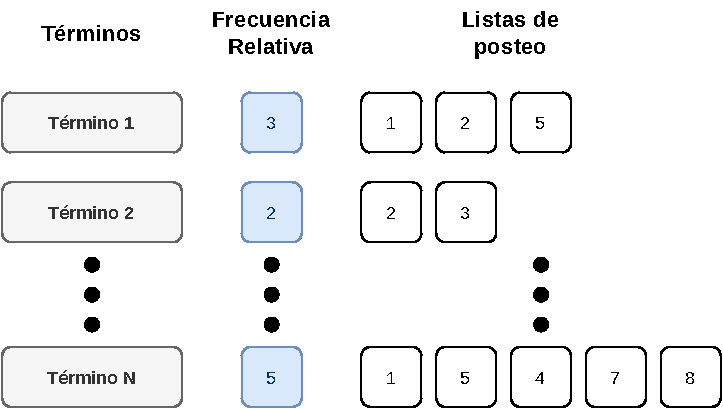
\includegraphics[width=0.7\textwidth]{images/BSII/II.pdf}
    \caption{Representación de un índice invertido. Se puede evidenciar una serie de términos al cual se asocia su frecuencia relativa y una lista de posteo con los identificadores de los documentos donde aparecen.}
    \label{fig:inverted_index}
\end{figure}

\subsubsection{Construcción del Índice Invertido}
Según \cite{IR-book} existen cuatro estrategias principales para construir eficientemente un índice invertido de búsqueda binaria (BSII, \textit{Binary Search Inverted Index}. La selección de una es estas estrategias depende de las características del hardware sobre el cuál vaya a ser implementada, especialmente en lo que se refiere al número de máquinas que van a ejecutar el algoritmo. 

Vale la pena mencionar que algunos de los valores presentados en \cite{IR-book} incluyen valores y consideraciones propias de sistemas típicos de 2007. Es necesario tener en cuenta que desde 2007 hasta la actualidad (2021) se han presentado avances de hardware que pueden afectar los algoritmos de construcción del índice invertido y búsqueda de información.

Las estrategias para construir el índice invertido son: indexado basado en ordenamiento en bloques (BSBI, \textit{Blocked Sort-Based Indexing}), indexado en memoria de un solo paso (SPIMI, \textit{Single-Pass In-Memory Indexing}), indexado distribuido e indexado dinámico. Tanto el BSBI como el SPIMI están contemplados como estrategias para ser usadas en una máquina, mientras que el indexado distribuido y el indexado dinámico suelen ser usados en grupos de máquinas. 

Dado que la solución del enunciado debe ser realizada exclusivamente en una máquina, debido al tamaño de la base de datos y la disponibilidad de recursos, solo serán revisadas las estrategias de BSBI y SPIMI. Las dos estrategias están contempladas para realizar un único paso por los datos para construir el índice.

\paragraph{Indexado Basado en Ordenamiento en Bloques (BSBI)} Esta estrategia es utilizada para construir el índice invertido dividiendo la colección en bloques de igual tamaño que son analizadas en memoria. Para cada bloque se realiza el siguiente proceso:

\begin{enumerate}
    \item Se recupera el siguiente bloque de la colección.
    \item El bloque es procesado para extraer parejas de identificador del término e identificador del documento (\textit{termID} - \textit{docID}).
    \item Se invierten el bloque para construir un resultado intermedio del índice invertido. El resultado de este proceso es que para un identificador de un término se tendrá una lista con los identificadores de los documentos en los que aparece.
    \item Los resultados intermedios para cada bloque son almacenados temporalmente en el almacenamiento secundario.
    \item Una vez se han invertido todos los bloques de la colección, los resultados intermedios se unen en lo que será el índice invertido.
\end{enumerate}

La idea de dividir la colección en bloques de igual tamaño tiene el propósito de realizar lecturas contiguas en el almacenamiento secundario. De esta manera, los tiempos de lectura son inferiores a lo que sería una serie lecturas aleatorias en el disco.

Un factor crítico de esta estrategia es el procesamiento del texto para la extracción de las parejas de identificadores de términos y documentos. La estructura de datos que realiza la relación entre término y su identificador podría llegar a ocupar una gran cantidad de espacio de memoria para colecciones lo suficientemente grandes. Esta situación se corrige con la estrategia SPIMI. 

\paragraph{Indexado en Memoria de un Solo Paso (SPIMI)}
La estrategia SPIMI busca construir el índice invertido a partir de los términos directamente. El objetivo de SPIMI consiste en crear un diccionario de forma dinámica conforme se van leyendo las parejas de término e identificador del documento. De forma general, el algoritmo de SPIMI realiza el siguiente proceso:

\begin{enumerate}
    \item Se crea un archivo de salida y un diccionario. El archivo de salida será usado para almacenar los resultados intermedios. En este caso, el resultado intermedio será el diccionario.
    \item Se va iterando sobre cada pareja de término e identificador del documento. Si el término está en el diccionario, se recupera la su entrada y se agrega el nuevo identificador de documento. Se lo contrario, se agrega la entrada en el documento. 
    \item Cuando la memoria se llena, se organizan los términos del diccionario con un orden lexicográfico y se escriben en el almacenamiento secundario.
    \item Una vez se han procesado todas las parejas, se realiza la unión de los diccionarios para obtener el índice invertido.
\end{enumerate}

Una de las ganancias que se obtiene al utilizar la estrategia SPIMI en comparación al BSBI es que no es necesario ordenar las parejas de términos e identificadores de documentos durante la construcción del índice. Otro beneficio consiste en que, como se indicó previamente, SPIMI no requiere de una estructura de datos que asocie un término con su identificador, por lo que la memoria principal puede ser usada eficientemente.

\subsubsection{Gestión de Recursos y Acceso a Memoria}
Dado que un índice invertido puede ser una estructura que ocupe una gran cantidad de espacio de almacenamiento, es necesario establecer estrategias con el fin de que dicha estructura sea accesible de forma eficiente y que requiera menos almacenamiento. En primer lugar, es necesario prevenir que el índice va a ser guardado en el almacenamiento secundario ya que es probable que ocupe más espacio del provisto por la memoria principal. En este orden de ideas deben solucionarse dos situaciones: el índice debe ser accedido en el almacenamiento secundario de forma rápida y debe ocupar el menor espacio posible.

Para disminuir el tiempo de acceso al índice es posible hacer uso de la jerarquía de memoria y el principio de localidad para cachear (\textit{caching}) las listas de posteo en la memoria principal. De esta manera se reduce el tiempo de acceso al índice para los términos que se usan con mayor frecuencia. Por otra parte, se pueden utilizar algoritmos de compresión y descompresión con el fin de disminuir el espacio de almacenamiento requerido para el índice. El uso de dichos algoritmos tiene dos beneficios: reduce el espacio utilizado en el almacenamiento secundario y permite incluir más términos en la memoria principal.

Es necesario considerar que un índice está compuesto por el vocabulario y las listas de posteo, donde el primero ocupa un espacio de almacenamiento considerablemente menor al segundo. En este contexto, es necesario establecer estrategias diferentes de compresión dependiendo de si el elemento a comprimir es el vocabulario o las listas de posteo. Para comprimir el diccionario se pude recurrir a codificarlo como una cadena de caracteres donde se incluya el término, su frecuencia relativa y un puntero a su lista de posteo. Esta estrategia de compresión puede se complementada con un agrupamiento de los términos en bloques de un tamaño definido. Al implementar estas dos estrategias de compresión es posible reducir la cantidad de almacenamiento requerido por el diccionario. Sin embargo, el tiempo de acceso para este puede verse afectado, especialmente al implementar el agrupamiento. 

El caso de las listas de posteo tiene mayor incidencia en el tamaño del diccionario dado que corresponden a la mayor parte de los datos que deben ser almacenados. En primer lugar, es necesario tener en cuenta que las listas de posteo se pueden definir como el identificador de un documento inicial y una serie de incrementos relativos a este. En este sentido, es posible codificar dichos incrementos como una serie de valores de tamaño dinámico en contraposición a valores de tamaño fijo. De esta manera se puede garantizar que el almacenamiento empleado para codificar los incrementos sean usados eficientemente. Existen dos estrategias para codificar dichos incrementos de forma dinámica: codificar a nivel de bytes y a nivel de bits. 

\subsubsection{Solución de Consultas al Índice Invertido}
Una consulta al índice invertido permite realizar búsquedas binarias usando los operadores lógicos AND, OR y NOT. Por una parte se tiene que dos términos con conjuntivos si se relacionan mediante un operador AND y disjuntos si se relacionan con un operador OR. Con el fin de resolver una consulta al índice invertido es necesario recuperar las listas de posteo de los dos términos y realizar la intersección de las dos listas según el operador lógico usado. Naturalmente, en caso que algún término sea modificado mediante el operador NOT, es necesario establecer el complemento de la lista de posteo de dicho término. Una vez se ha realizado la intersección de las dos listas se puede retornar el resultado o continuar con los demás términos de la consulta.

Un aspecto clave de la consulta a un índice invertido es la intersección entre dos listas de posteo. En [1] se presenta un algoritmo de intersección para dos listas de posteo con un operador de conjunción (AND). Sin embargo, este debe modificarse para que pueda incluir una intersección disjunta (OR) y un operador de modificación (NOT). El listado \ref{lst:intersect} presenta el algoritmo para realizar la intersección de dos listas de posteo con operadores conjuntivos, disjuntos y de modificación.

\begin{lstlisting}[
    basicstyle=\scriptsize,
    caption={Algoritmo para la intersección de listas de posteo con operadores conjuntivos, disjuntos y de modificación.}, 
    label=lst:intersect, 
    captionpos=b,
    abovecaptionskip=1em,
    belowcaptionskip=1em
]
INTERSECT(p1, p2, op, mod1, mod2, n):
    if mod1 == NOT do
        p1 = complement(p1, n)
    
    if mod2 == NOT do
        p2 = complement(p2, n)
        
    if length(p2) < length(p1) do
        p1, p2 = p2, p1
        
    answers = []
    indexes = [0, 0]
    finish = false
    
    while not finish do
        posting1 = p1[indexes[0]]
        posting2 = p2[indexes[1]]
    
        if operator == AND do
            if posting1 == posting2 do
                append(answers, posting1)
                
            if posting1 < posting2 do
                increment(indexes[0])
            else do
                increment(indexes[0])
                
            if indexes[0] == length(p1) and indexes[1] == length(p2) do
                finish = true
        
        else do
            if indexes[0] != length(p1) do
                if posting1 < posting2 do
                    append(answers, posting1)
                    increment(indexes[0])
                
                else if posting1 == posting2 do
                    append(answers, posting1)
                    increment(indexes[0])
                    increment(indexes[1])
                    
                else do
                    append(answers, posting2)
                    increment(indexes[1])
                    
            else do
                append(answers, posting2)
                increment(indexes[1])
                
            if indexes[1] == length(p2) do
                finish = true
        
\end{lstlisting}

En la ejecución del algoritmo presentado en el listado \ref{lst:intersect} se realizan los siguientes pasos:

\begin{itemize}
    \item Se realiza la modificación (\texttt{mod1}, \texttt{mod2}) de las listas de posteo (\texttt{p1} y \texttt{p2}) dependiendo del número de documentos presentes en la colección (\texttt{n}). Se asume que los identificadores de los documentos hacen parte de un conjunto de enteros que van desde el número uno hasta \texttt{n}.
    \item Se organizan las listas de posteo de modo tal que \texttt{p1} apunte a la lista de menor tamaño y \texttt{p2} apunte a la lista de mayor tamaño.
    \item Se crea un arreglo vacío para almacenar las respuestas y otro con dos enteros que almacenan los índices para las listas de posteo.
    \item Se itera mientras que no se haya alcanzado la condición de parada. En primer lugar se recuperan los elementos de las listas de posteo según los índices almacenados en el arreglo correspondiente. Dependiendo del operador (\texttt{op}) se realizan las siguientes acciones dentro del ciclo:
    
    \begin{itemize}
        \item Si se trata de una intersección conjuntiva se revisa si los dos elementos son iguales. En caso que sean iguales se agregan al arreglo de respuestas. Se incrementa el índice del elemento que corresponda al menor valor. Cuando los dos índices alcancen la longitud de la lista se activa la condición de parada.
        \item Si se trata de una intersección disjunta se revisa si el primer índice no haya alcanzado la longitud de la primera lista de posteo. Si el elemento de la primera lista es inferior al elemento de la segunda, el primer elemento es agregado al arreglo de respuestas y el índice de la primera lista incrementado. En caso tal que los dos elementos sean iguales, uno de estos se agrega a la lista de respuestas y los dos índices se incrementan. Finalmente, si el elemento de la segunda lista es mayor, este es agregado a las respuestas y su índice es aumentado. En caso tal que el primer índice haya alcanzado la longitud de su lista correspondiente, se agregan los elementos restantes de la segunda lista al arreglo de respuestas. Cuando se han agregado todos los elementos de la segunda lista se agrega la condición de parada.
    \end{itemize}
\end{itemize}

Si una consulta contiene más de dos términos es necesario establecer una estrategia para optimizar la recuperación de las listas de posteo y su intersección. Una de las estrategias con mayor adopción consiste en organizar la intersección de las listas según la frecuencia relativa de los términos. No obstante, esta estrategia de implementación es válida para las intersecciones conjuntivas. Es necesario modificar la estrategia levemente con el fin de incluir tanto las operaciones disjuntas. En este orden de ideas, una estrategia sería resolver las operaciones disjuntas en orden incremental antes de resolver las operaciones disjuntas.


\subsubsection{Implementación}
Teniendo en cuenta que la implementación se haría en Python y que esta sería ejecutada en una máquina, se podría partir de la estrategia SPIMI para construir el índice invertido. Esta decisión se toma en base a las siguientes consideraciones:

\begin{itemize}
    \item SPIMI no requiere un mayor control sobre la memoria principal como sí lo requiere BSBI. Dado que Python no ofrece métodos para realizar este control, dado que es un lenguaje de alto nivel, se favorece la implementación de SPIMI sobre BSBI.
    \item Python ofrece diccionarios de forma nativa. Estos diccionarios pueden contener como llave (\textit{key}) la cadena de texto del término en cuestión y como valor (\textit{value}) una lista con los identificadores del documento.
    \item Con la implementación de listas nativas de Python no es necesario alocar memoria directamente desde el algoritmo. Python hace esto sin que el programador deba indicarlo explícitamente.
\end{itemize}

Aprovechando dicha estrategia se tiene que el conjunto de datos es almacenado enteramente en la memoria, por lo que no es necesario implementar una estrategia de lectura en el almacenamiento secundario. En este sentido, la implementación lee los documentos del conjunto de datos de modo tal que se cree una pareja con el término y el identificador del documento. Inicialmente se tiene un diccionario cuya llave (\textit{key}) es el término y el valor (\textit{value}) corresponde a una lista donde se van agregando los identificadores de los documentos. Una vez se han procesado todos los documentos se convierte dicho diccionario en una matriz de Numpy que es almacenada en disco para su uso posterior.  



